% Leakage-control timeline shared by the Elsevier and IEEE entry points.
\usetikzlibrary{arrows.meta,positioning}

\begin{figure*}[!t]
\centering
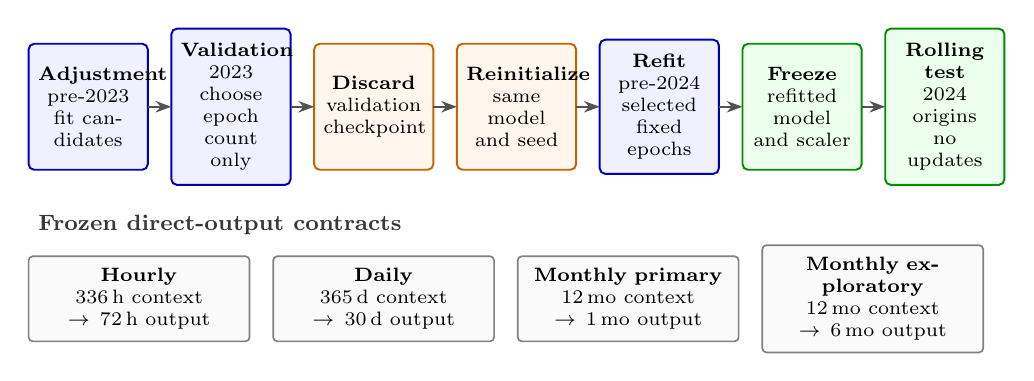
\begin{tikzpicture}[
  font=\scriptsize,
  timeline step/.style={
    rounded corners=2pt,
    line width=0.7pt,
    text width=0.105\textwidth,
    minimum height=16mm,
    align=center,
    inner xsep=1.2mm,
    inner ysep=1.8mm,
    outer sep=0pt
  },
  data step/.style={
    timeline step,
    draw=blue!72!black,
    fill=blue!6
  },
  reset step/.style={
    timeline step,
    draw=orange!78!black,
    fill=orange!7
  },
  locked step/.style={
    timeline step,
    draw=green!55!black,
    fill=green!7
  },
  timeline arrow/.style={
    -{Stealth[length=2.0mm,width=1.45mm]},
    draw=black!68,
    line width=0.75pt
  },
  contract/.style={
    draw=black!50,
    fill=black!2,
    rounded corners=1.5pt,
    line width=0.6pt,
    text width=0.205\textwidth,
    minimum height=9mm,
    align=center,
    inner xsep=1.6mm,
    inner ysep=1.5mm,
    outer sep=0pt
  }
]

\node[data step] (adjustment) {
  \textbf{Adjustment}\\
  pre-2023\\
  fit candidates
};
\node[data step,right=3mm of adjustment] (validation) {
  \textbf{Validation}\\
  2023\\
  choose epoch count only
};
\node[reset step,right=3mm of validation] (discard) {
  \textbf{Discard}\\
  validation\\
  checkpoint
};
\node[reset step,right=3mm of discard] (reinitialize) {
  \textbf{Reinitialize}\\
  same model\\
  and seed
};
\node[data step,right=3mm of reinitialize] (refit) {
  \textbf{Refit}\\
  pre-2024\\
  selected fixed epochs
};
\node[locked step,right=3mm of refit] (freeze) {
  \textbf{Freeze}\\
  refitted model\\
  and scaler
};
\node[locked step,right=3mm of freeze] (test) {
  \textbf{Rolling test}\\
  2024 origins\\
  no updates
};

\draw[timeline arrow] (adjustment.east) -- (validation.west);
\draw[timeline arrow] (validation.east) -- (discard.west);
\draw[timeline arrow] (discard.east) -- (reinitialize.west);
\draw[timeline arrow] (reinitialize.east) -- (refit.west);
\draw[timeline arrow] (refit.east) -- (freeze.west);
\draw[timeline arrow] (freeze.east) -- (test.west);

\node[anchor=north west,font=\footnotesize\bfseries,text=black!78]
  (contracts-title) at ([yshift=-4.5mm]adjustment.south west)
  {Frozen direct-output contracts};

\node[contract,anchor=north west] (hourly)
  at ([yshift=-1.5mm]contracts-title.south west) {
    \textbf{Hourly}\\
    $336\,\mathrm{h}$ context $\rightarrow 72\,\mathrm{h}$ output
  };
\node[contract,right=3mm of hourly] (daily) {
    \textbf{Daily}\\
    $365\,\mathrm{d}$ context $\rightarrow 30\,\mathrm{d}$ output
  };
\node[contract,right=3mm of daily] (monthly-one) {
    \textbf{Monthly primary}\\
    $12\,\mathrm{mo}$ context $\rightarrow 1\,\mathrm{mo}$ output
  };
\node[contract,right=3mm of monthly-one] (monthly-six) {
    \textbf{Monthly exploratory}\\
    $12\,\mathrm{mo}$ context $\rightarrow 6\,\mathrm{mo}$ output
  };

\end{tikzpicture}
\caption{Temporal selection, refit, and evaluation protocol for each neural
model--seed pair. Blue boxes fit or score on historical partitions, orange
boxes enforce fresh retraining, and green boxes denote the locked test state.
XGBoost follows the analogous separation with a fixed tree budget and
independently fitted adjustment and refit instances. Each rolling origin emits
the complete direct horizon shown in the lower band.}
\label{fig:temporal_protocol}
\end{figure*}
